\chapter{Prehľad existujúcich riešení}
Aj keď oblasť budíkov je každému dobre známa, napriek tomu sme sa rozhodli vytvoriť prehľad existjúcich riešení, ktoré môžme využiť ako inšpiráciu pri našej práci.

\section{Tradičné analógové budíky}
Analógové, alebo ručičkové budíky majú väčšinou na vrchu dva zvončeky, medzi ktorými kmitá srdiečko. Jeho rýchle údery spôsobujú známy pravidelný zvuk. Takéto budíky obsahujú tri ručičky, z toho dve sú na ukazovanie času a tretia na nastavenie času, v ktorom sa má ozvať budiaci tón.

\begin{figure}[h]
    \centering
    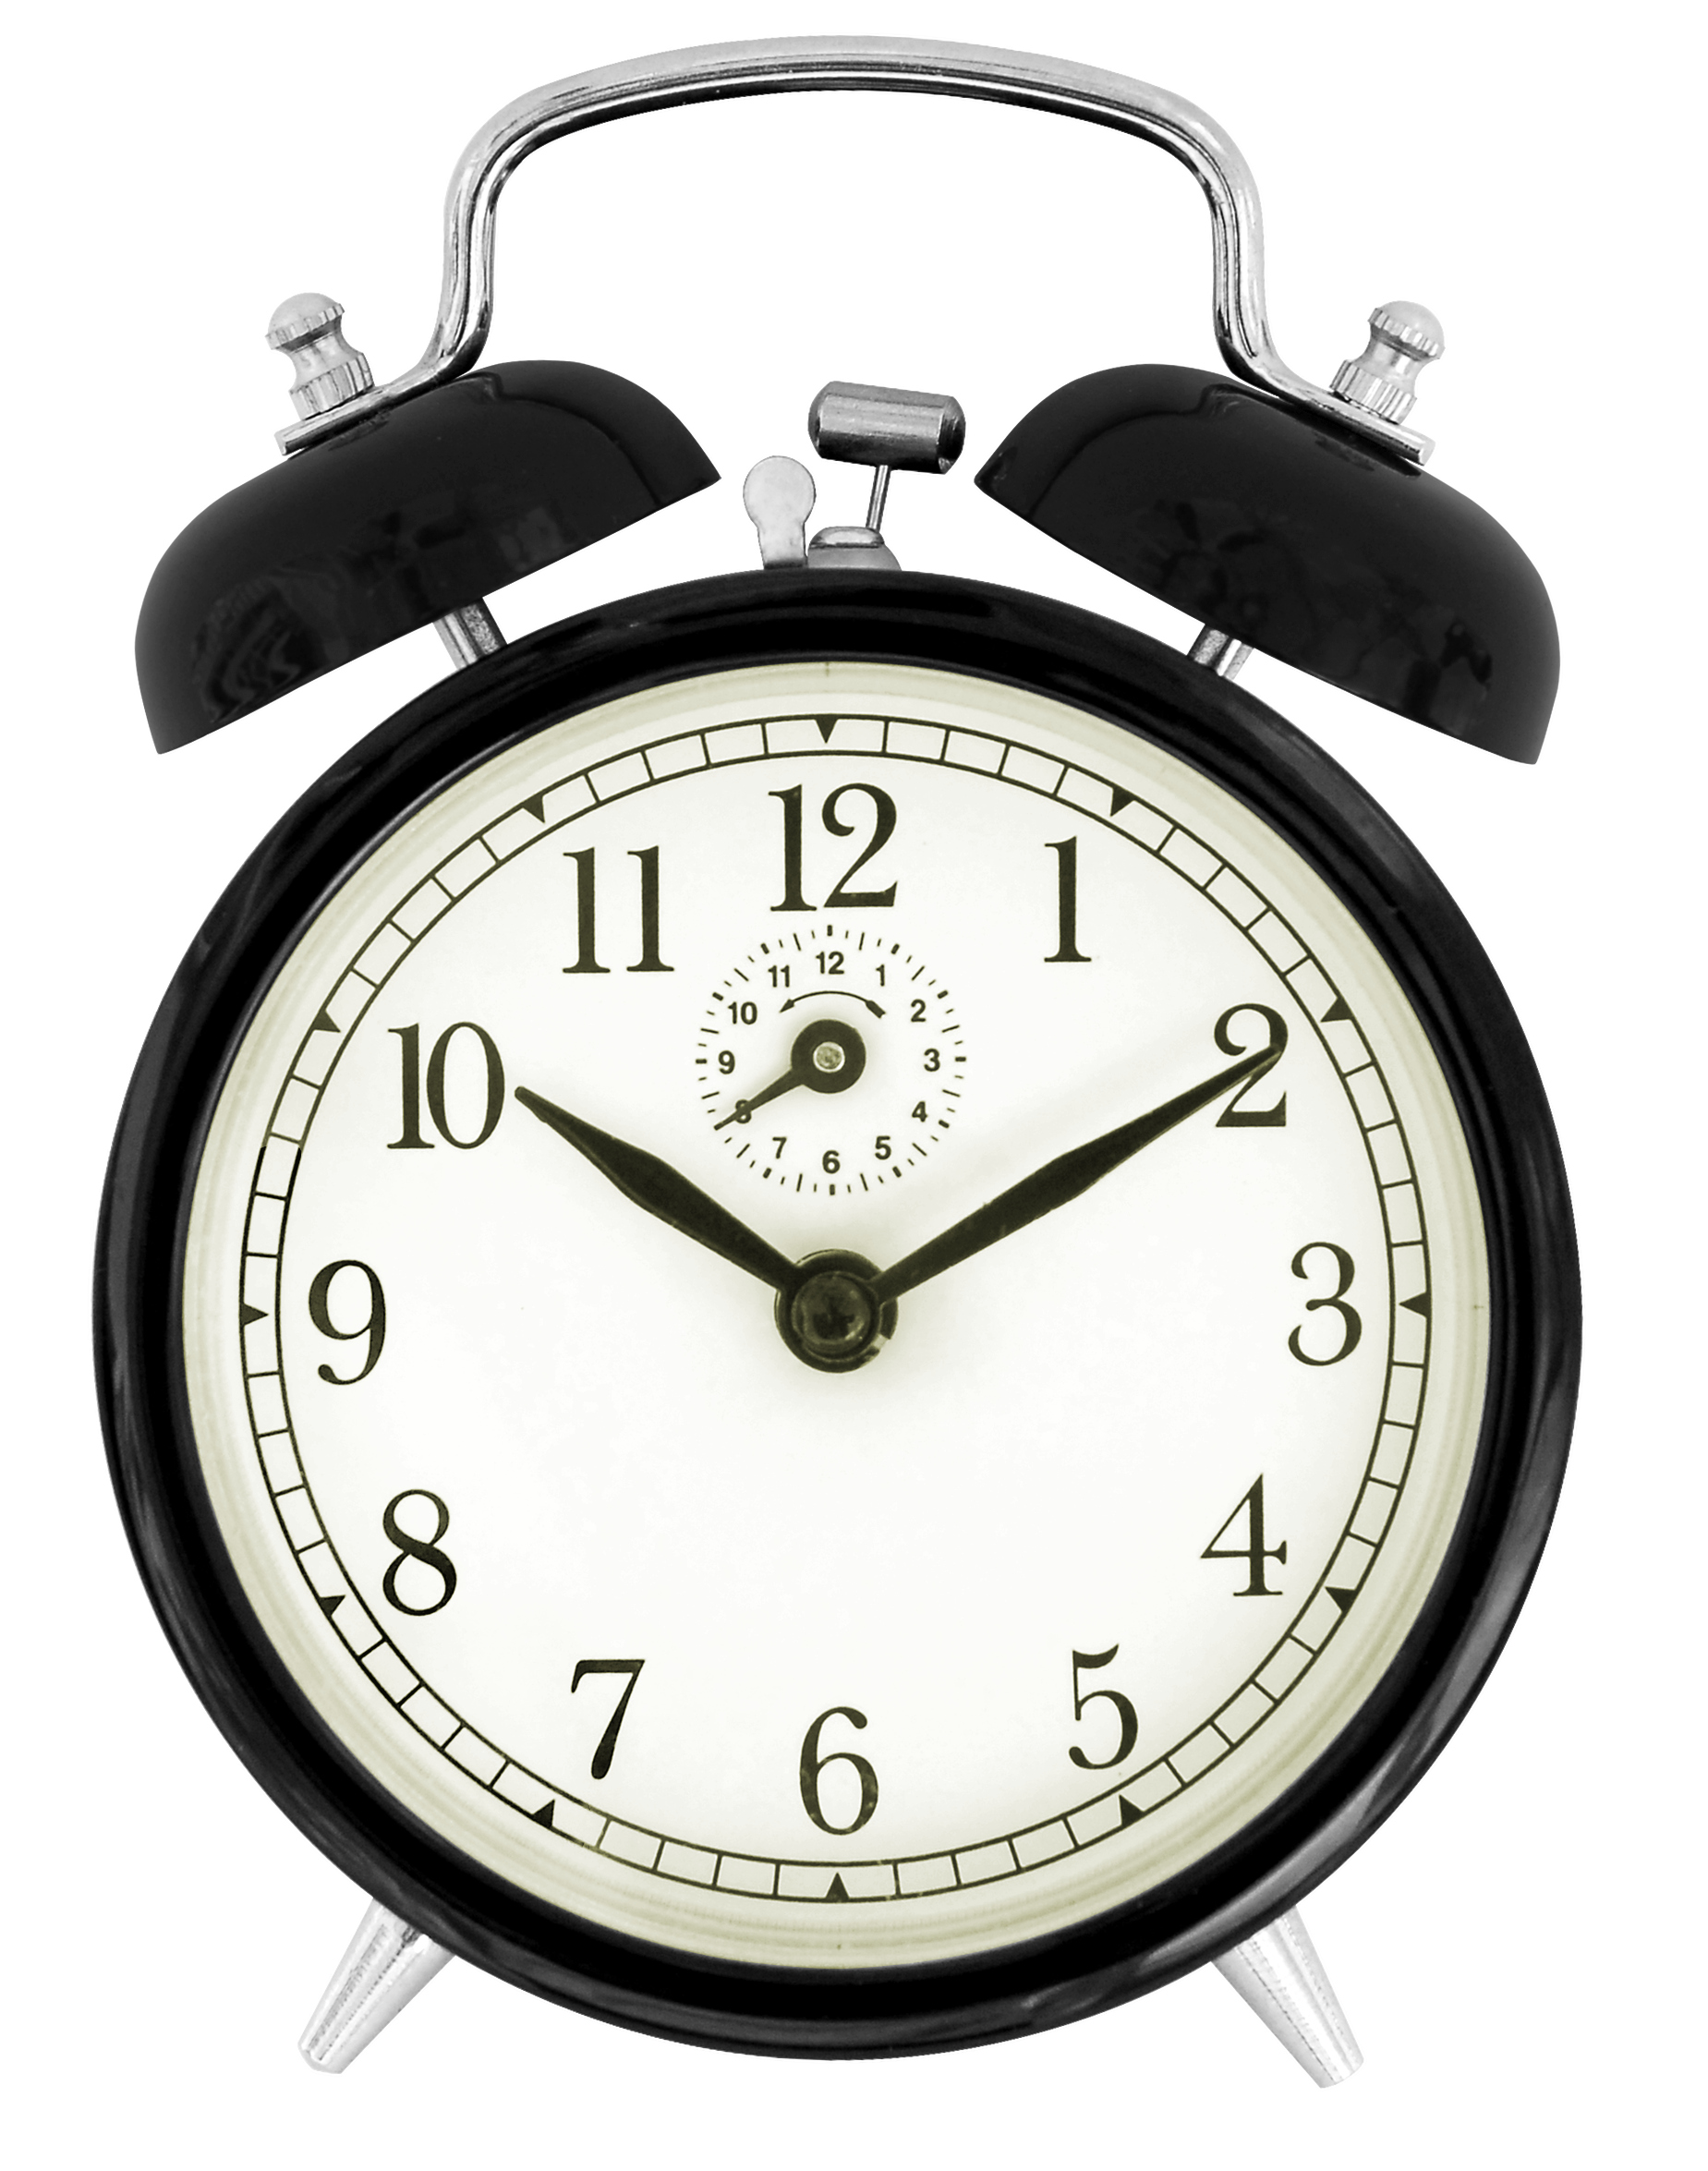
\includegraphics[width=0.4\textwidth]{img/analog.jpg}
    \caption{Tradičný analógový budík.}
\end{figure}

Nevýhodou takýchto budíkov je, že sa nadajú nastaviť tak, aby zvonli po viac ako dvanástich hodinách. Ručičky sa ovládalú zo zadnej strany budíku, kde sa nachádzajú rotačné páčky~\cite{hodkin-2015}.

\section{Digitálne budíky}
Digitálne budíky využívajú na vytváranie zvuku menší reproduktor, pomocou ktorého vydáva pravidelý alebo nepravidelný zvuk. Číslice na budíku sú znázornené na digitálnom dispjeli najčastejšie arabskými číslicami od 00:00:00 do 23:59:59. Nastavuje sa väčšinou pomocou tlačítok~\cite{hodkin-2015}.

\begin{figure}[h]
    \centering
    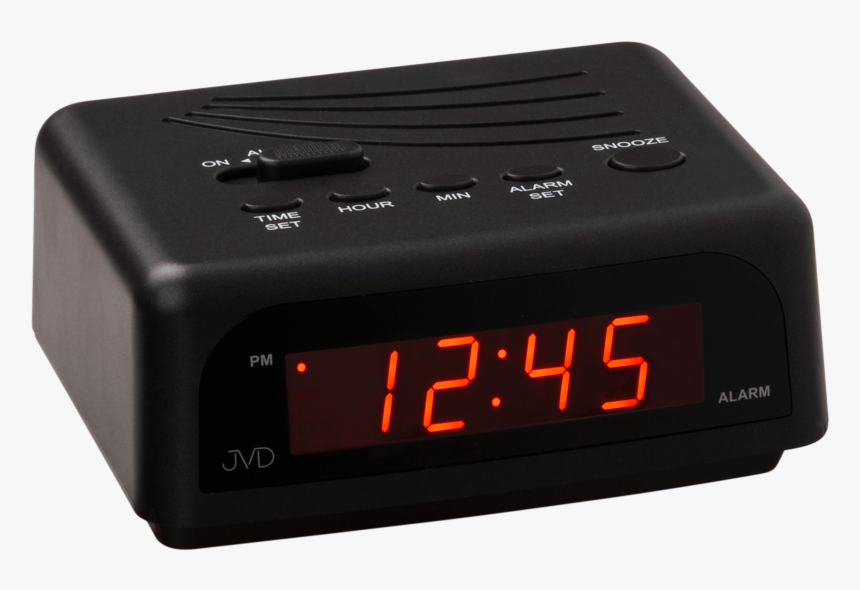
\includegraphics[width=0.6\textwidth]{img/digi.png}
    \caption{Digitálny budík.}
\end{figure}

\section{Rádiobudíky}
Rádiobudíky sú budíky a rádiopríjmače intefrované do jedného zariadenia. Takéto budíky môžu v určený čas zapnúť rádio, ktoré bude slúžiť na budenie. Novšie modely podporujú iné zdroje hudby, napríklad mobilný telefón alebo CD.

\section{Mobilné telefóny}
Väčšina ľudí dnes používa na budenie mobilný telefón.
Veľa mobilných telefónov obsahuje vstavaný budík, ktorý nevyžaduje, aby bol mobilný telefón zapnutý. Typickou funkciou takéhoto budíku je možnosť vybrať vlastný tón budenia~\cite{mb-clock}.
%\section{Budíky novej generácie}
